\section{Компилиране за различни платформи}
За да компилирате Rust за различни платформи, ще трябва да инсталирате
toolchain и след това компилираме проекта. За да видим различните видове
toolchain-и, можем да използваме следната команда:
\begin{lstlisting}
rustup target list
\end{lstlisting}
Тази команда ще изведе имената за над 90 различни поддържани платформи, но ще
се фокусираме само върху Windows и Linux. Те отговарят на имената
"x86-64-pc-windows-gnu" и "x86\_64-unknown-linux-gnu".

За автоматичното компилиране и архивиране на файловете за различните платформи
можем да създадем един Bash скрипт [Фигура \ref{fig:cross-compile}]. Този
скрипт автоматично ще инсталира toolchain-a ако вече не е, компилира проекта и
създава zip архив със файла за изпълнение.

\begin{figure}[!htb]
  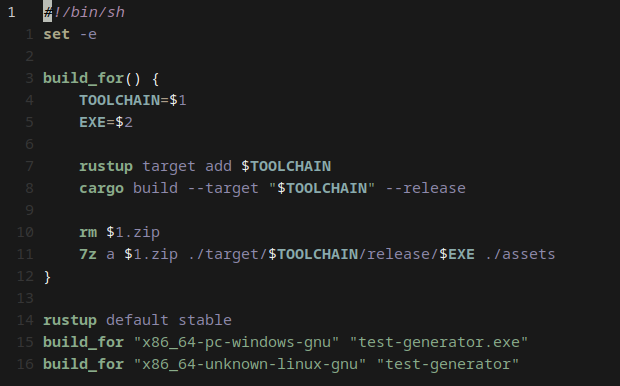
\includegraphics[scale=0.75]{cross-compile.png}
  \centering
  \caption{Bash скрипт за комилиране и архивиране на проекта}
  \label{fig:cross-compile}
\end{figure}

На 3ти ред във Фигура \ref{fig:cross-compile} дефинираме функция
\textit{build\_for} която приема като аргумени името на toolchain-a и името на
компилирания файл. Функцията компилира и проекта използвайки всички оптимизации
и го архивира във файл със същотот име като името на toolchain-a.

Тези архиви могат да бъдат разпространени в интернет и всеки потребител да
изтегли съответната версия за неговата платформа и да използва софтуерния
продукт.
